

\documentclass[border=0.125cm]{standalone}
\usepackage{tikz,ifthen,calc}
\usetikzlibrary{positioning}
\begin{document}

\tikzset{%
  every neuron/.style={
    circle,
    draw,
    minimum size=1cm
  },
  neuron missing/.style={
    draw=none, 
    scale=4,
    text height=0.333cm,
    execute at begin node=\color{black}$\vdots$
  },
}

\tikzset{fontscale/.style = {font=\relsize{#1}}
    }

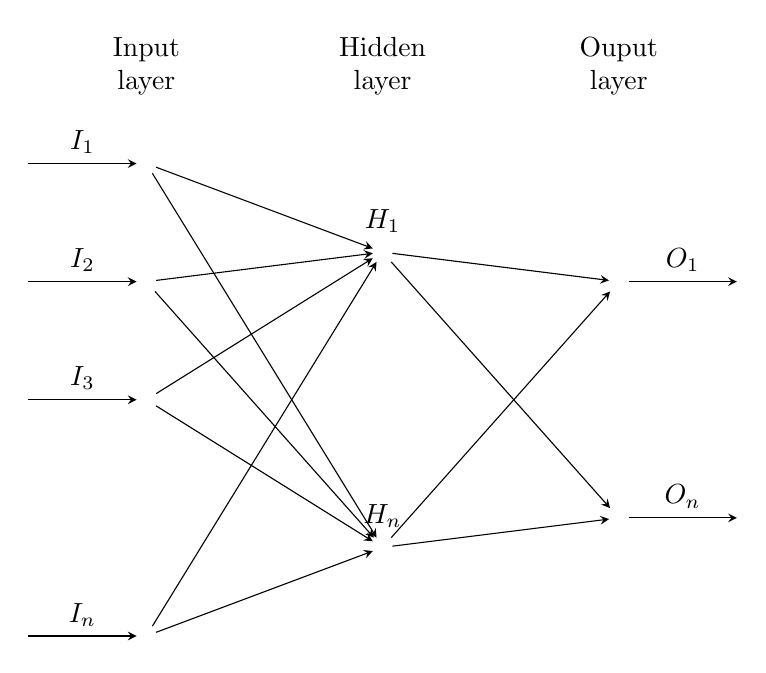
\begin{tikzpicture}[x=1.5cm, y=1.5cm, >=stealth]

\foreach \m/\l [count=\y] in {1,2,3,missing,4}
  \node [every neuron/.try, neuron \m/.try] (input-\m) at (0,2.5-\y) {};

\foreach \m [count=\y] in {1,missing,2}
  \node [every neuron/.try, neuron \m/.try ] (hidden-\m) at (2,2-\y*1.25) {};

\foreach \m [count=\y] in {1,missing,2}
  \node [every neuron/.try, neuron \m/.try ] (output-\m) at (4,1.5-\y) {};

\foreach \l [count=\i] in {1,2,3,n}
  \draw [<-] (input-\i) -- ++(-1,0)
    node [above, midway] {$I_\l$};

\foreach \l [count=\i] in {1,n}
  \node [above] at (hidden-\i.north) {$H_\l$};

\foreach \l [count=\i] in {1,n}
  \draw [->] (output-\i) -- ++(1,0)
    node [above, midway] {$O_\l$};

\foreach \i in {1,...,4}
  \foreach \j in {1,...,2}
    \draw [->] (input-\i) -- (hidden-\j);

\foreach \i in {1,...,2}
  \foreach \j in {1,...,2}
    \draw [->] (hidden-\i) -- (output-\j);

\foreach \l [count=\x from 0] in {Input, Hidden, Ouput}
  \node [align=center, above] at (\x*2,2) {\l \\ layer};

\end{tikzpicture}

\def\nInput{4}
\def\nHidden{2}
\def\nHLayers{2}
\def\nOutput{2}
\begin{tikzpicture}[x=1.5cm, y=1.5cm, >=stealth]

% Create Nodes
% Input layer nodes
\foreach \m/\l [count=\y] in {1,2,missing,\nInput}
  \node [every neuron/.try, neuron \m/.try] (input-\m) at (0,2.5-\y) {};

% hideen layer nodes
\foreach \m [count=\y] in {1,missing,\nHidden}
  \node [every neuron/.try, neuron \m/.try ] (hiddena-\m) at (3,2-\y*1.25) {};
  
\foreach \m [count=\y] in {1,missing,\nHidden}
  \node [every neuron/.try, neuron \m/.try ] (hiddenb-\m) at (6,2-\y*1.25) {};

% Output layer nodes
\foreach \m [count=\y] in {1,missing,\nOutput}
  \node [every neuron/.try, neuron \m/.try ] (output-\m) at (9,1.5-\y) {};

% Label First Hidden Layer Nodes
\foreach \l [count=\i] in {1,2, b,n}
  \node [above] at (input-\i.west) {$I_\l$};

% Label First Hidden Layer Nodes
\foreach \l [count=\i] in {1,n}
  \node [above] at (hiddena-\i.north) {$H_\l$};
  
% Label Second Hidden Layer Nodes
\foreach \l [count=\i] in {1,n}
  \node [above] at (hiddenb-\i.north) {$H_\l$};
  
% Label Second Hidden Layer Nodes
\foreach \l [count=\i] in {1,n}
  \node [above] at (output-\i.east) {$O_\l$};

%% Draw Arrows 
% from hidden layer a to input
\foreach \i in {1,...,\nInput}
  \foreach \j in {1,...,\nHidden}
    \draw [<-] (input-\i) -- (hiddena-\j);
    
\foreach \i [count=\a] in {1,n} {
  \foreach \j [count=\b] in {1,n} {
  	\ifthenelse{\a=\b}{\def\posvar{.5}}{\def\posvar{.8}}
    \draw [->] (hiddenb-\a) -- (hiddena-\b) node[sloped, pos=\posvar, above, font=\tiny, scale=.5] {$w = w + \eta I\{3\}(\i) \delta$};
    }
}

\foreach \i [count=\a] in {1,n} {
  \foreach \j [count=\b] in {1,n} {
  	\ifthenelse{\a=\b}{\def\posvar{.5}}{\def\posvar{.75}}
    \draw [->] (hiddenb-\a) -- (hiddena-\b) node[sloped, pos=\posvar, below, font=\tiny, scale=.5] {$\delta = I\{3\}(\i)*(1 - I\{end\}(\i))*error$};
  }
}

\foreach \i [count=\a] in {1,n} {
  \foreach \j [count=\b] in {1,n} {
  	\ifthenelse{\a=\b}{\def\posvar{.5}}{\def\posvar{.7}}
    \draw [->] (hiddenb-\a) -- (hiddena-\b) node[sloped, pos=\posvar, yshift=-.1in, font=\tiny, scale=.5] {$error=?$};
  }
}
    
\foreach \i [count=\a] in {1,n} {
  \foreach \j [count=\b] in {1,n} {
  	\ifthenelse{\a=\b}{\def\posvar{.5}}{\def\posvar{.8}}
    \draw [->] (output-\a) -- (hiddenb-\b) node[sloped, pos=\posvar, above, font=\tiny, scale=.5] {$w = w + \eta I\{end\}(\i) \delta$};
    }
}

\foreach \i [count=\a] in {1,n} {
  \foreach \j [count=\b] in {1,n} {
  	\ifthenelse{\a=\b}{\def\posvar{.5}}{\def\posvar{.7}}
    \draw [->] (output-\a) -- (hiddenb-\b) node[sloped, pos=\posvar, below, font=\tiny, scale=.5] {$\delta = I\{end\}(\i)*(1 - I\{end\}(\i))*err$};
  }
}

\foreach \i [count=\a] in {1,n} {
  \foreach \j [count=\b] in {1,n} {
  	\ifthenelse{\a=\b}{\def\posvar{.5}}{\def\posvar{.7}}
    \draw [->] (output-\a) -- (hiddenb-\b) node[sloped, pos=\posvar, yshift=-.1in, font=\tiny, scale=.5] {$err=|target-value|$};
  }
}

% Label Layers
\foreach \l [count=\x from 0] in {Input \\ layer, Hidden \\ layer 1, Hidden \\ layer 2, Output \\ layer}
  \node [align=center, above] at (\x*3,2) {\l};

\end{tikzpicture}

\end{document}